%\documentclass[JIP,draft]{ipsj}
\documentclass[JIP]{ipsj}

\usepackage[dvips]{graphicx}
\usepackage{latexsym}

\def\Underline{\setbox0\hbox\bgroup\let\\\endUnderline}
\def\endUnderline{\vphantom{y}\egroup\smash{\underline{\box0}}\\}
\def\|{\verb|}

%\setcounter{volume}{20}% vol20=2012
%\setcounter{number}{4}% 1, 2, 3, 4
\setcounter{page}{1}

%\received{2011}{7}{1}
%\rereceived{2011}{10}{1}   % optional
%\rerereceived{2011}{10}{31} % optional
%\accepted{2011}{11}{5}

\usepackage[varg]{txfonts}%%!!
\makeatletter%
\input{ot1txtt.fd}
\makeatother%

\begin{document}

\title{Relaxing CDN Energy: Considering Peer-Assisted}

\affiliate{SFC}{Keio University Shonan Fujisawa Campus, 5322 Endo, Fujisawa-shi, Kanagawa 252-0882 Japan}

\author{Dikshie}{SFC}[dikshie@sfc.wide.ad.jp]
\author{Husni}{SFC}[husni@ai3.net]

\begin{abstract}
This paper presents an analysis of a peer-assisted CDN system, where an ISP manages its own CDN and its users participate in a P2P network to assist content delivery.
The system consists of a two-level CDN, where one level can be considered as the current CDN and the other level is managed by the ISP, and a number of user nodes forming a P2P network, where some of the user nodes are obliged to contribute in the content delivery.


\end{abstract}

\begin{keyword}
CDN, Data Center, Energy, Peer Assisted, P2P
\end{keyword}

\maketitle

%1
\section{Introduction}\label{intro}
Streaming content, especially video, represents a significant fraction of the traffic volume on the Internet, and it has become a standard practice to deliver this type of content using Content Delivery Networks (CDNs) such as Akamai and Limelight for better scaling and quality of experience for the end users.  
For example, Youtube uses Google cache and MTV uses Akamai in their operations.

With the spread of broadband Internet access at a reasonable flat monthly rate, users are connected to the Internet 24 hours a day and they can download and share multimedia content.  
P2P (peer to peer) applications are also widely deployed.  
In China, P2P is very popular; we see many P2P applications from China such as PPLive, PPStream, UUSe, Xunlei, etc.  
Some news broadcasters also rely on P2P technology to deliver popular live events.  
For example, CNN uses the Octoshape solution that enables their broadcast to scale and offer good video quality as the number of users increases.

From the Internet provider point of view, the presence of so many always-on users suggests that it is possible to delegate a portion of computing, storage and networking tasks to the users, thus creating P2P networks where users can share files and multimedia content.
Starting from file sharing protocols, P2P architectures have evolved toward video on demand and support for live events.

Broadband network access helps P2P applications to perform better.
xDSL networks are deployed worldwide, and in some countries, such as Japan, even higher bandwidth fiber to the home (FTTH) already exceeds DSL in market penetration.  In the coming years, FTTH will be massively deployed by network operators throughout the world.  
As access bandwidth increases, P2P systems may become more efficient since a peer can contribute much more.






\section{Motivation}\label{motivation}

\begin{figure}[tb]
\begin{center}
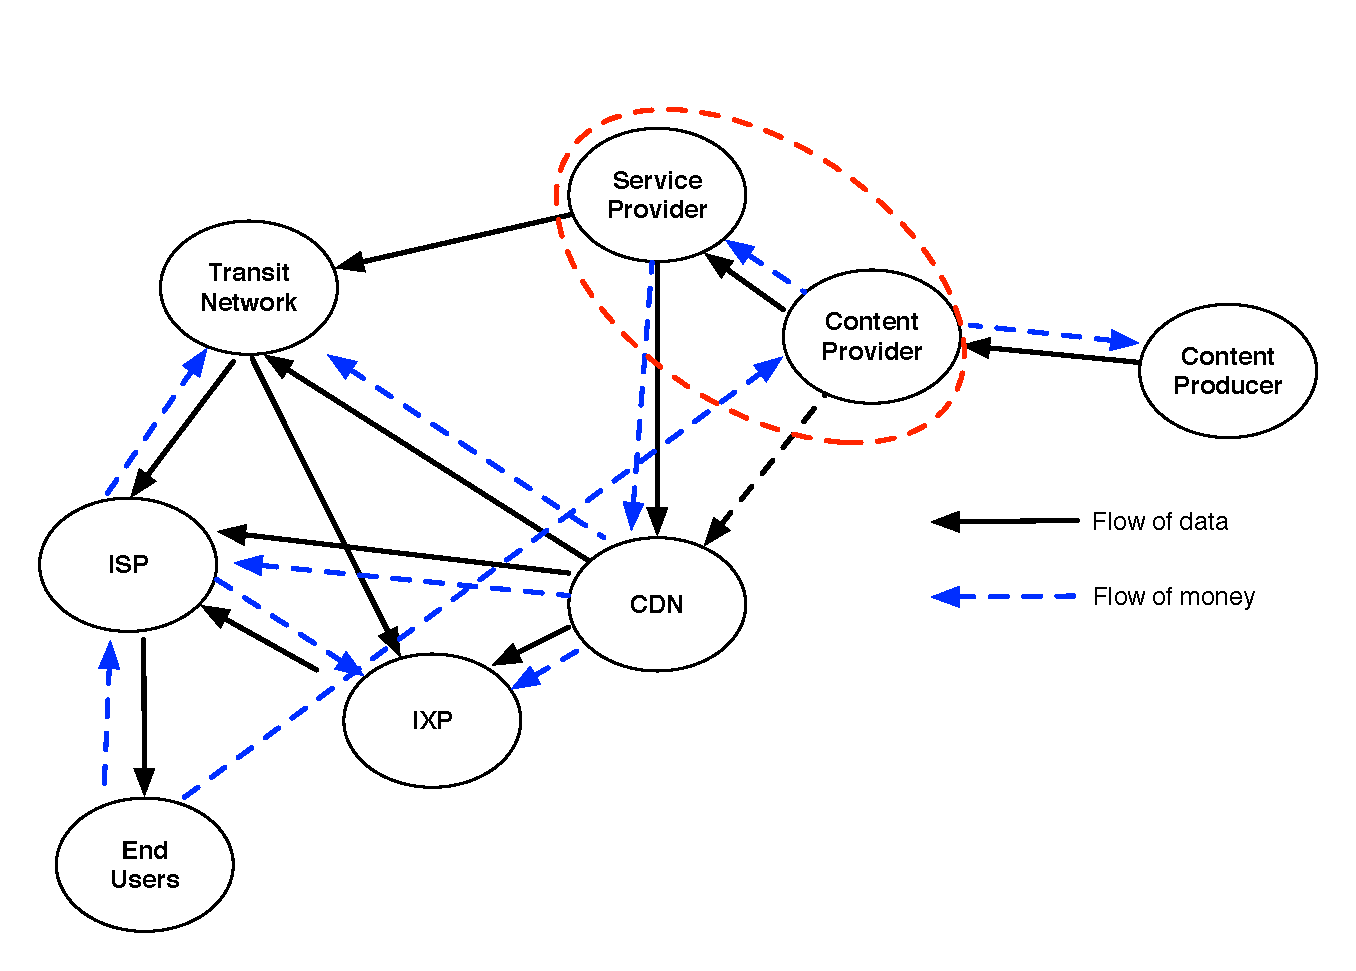
\includegraphics[scale=0.4]{graphs/business-relationship.eps}
\end{center}
\caption{Complex relationship of entities in Internet.
The data flow from content producer to content provider. 
Content producer such as movies companies send their movies to content provider for example: Netflix and Hulu.
Content providers then deliver the movies using CDN or they also can use their upstream provider.
Depends on routing and peering policy, data from CDN can flow directly to ISP or flow to ISP via IXP (Internet Exchange) or via transit network. 
Flow of data noted by straight arrow and flow of money noted by dash arrow line.
In current modern Internet topology, content provider and service provider can be merged in on entity, for example: Google.
Labovitz et al.,\cite{Labovitz:2010:IIT:2043164.1851194} mentioned that the hyper-giant entities such as Google doing massive peering to IXP in order to be closed to ISP. 
Although CDN is placed close to ISP network, it does not guarantee end-users can get good quality video stream \cite{Krishnan:2009:MBE:1644893.1644917}.
Other than technical complexity as mentioned before, CDN also faces economic complexity\cite{dispute}.
Therefore, the future of CDN business is likely to live deeper into ISP networks, more integrated into and interleaved with ISP infrastructures.}
\label{fig:businessrelationship}
\vspace{-2mm}
\end{figure} 

%\begin{figure}[thb]
%\begin{center}
%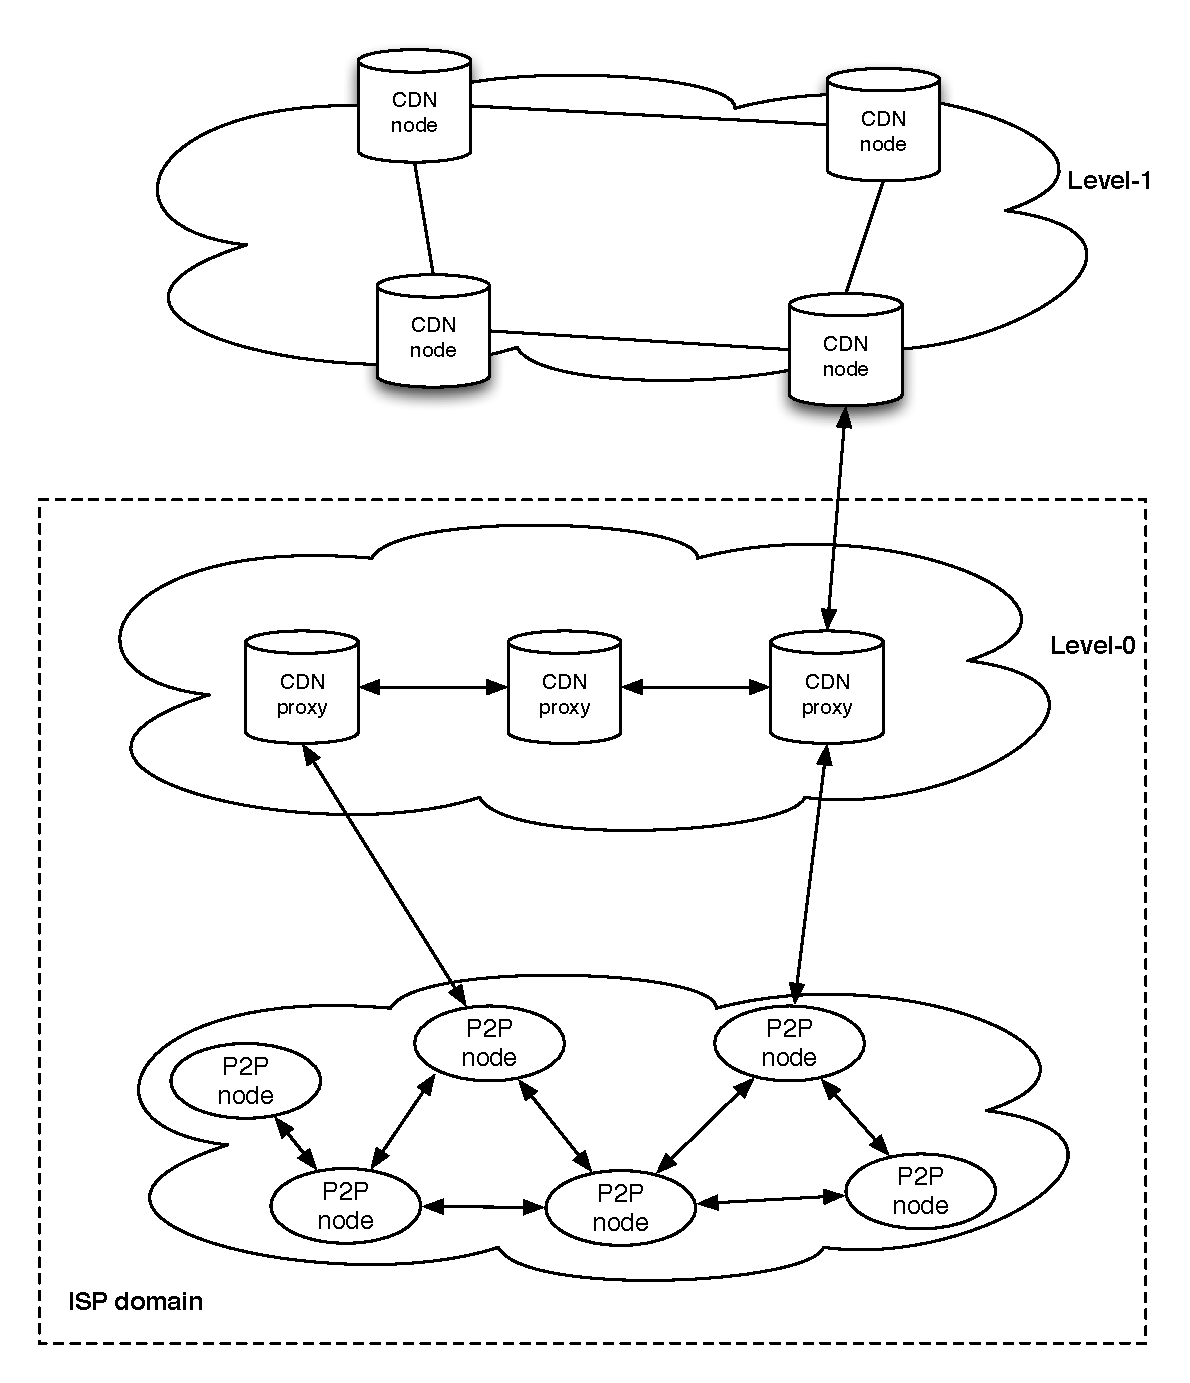
\includegraphics[scale=0.4]{graphs/two-tier-cdn-topology.eps}
%\end{center}
%\caption{Two tier CDN-P2P topology.
%The CDN proxy maintained by ISP. ISP also has CDN node. CDN node can exchange contents with other CDN node owned by other CDN companies.P2P nodes are ISP's customers %that run P2P software.}
%\label{fig:twotier}
%\vspace{-2mm}
%\end{figure} 



\section{System Model}\label{system model}

\begin{figure}[thb]
\begin{center}
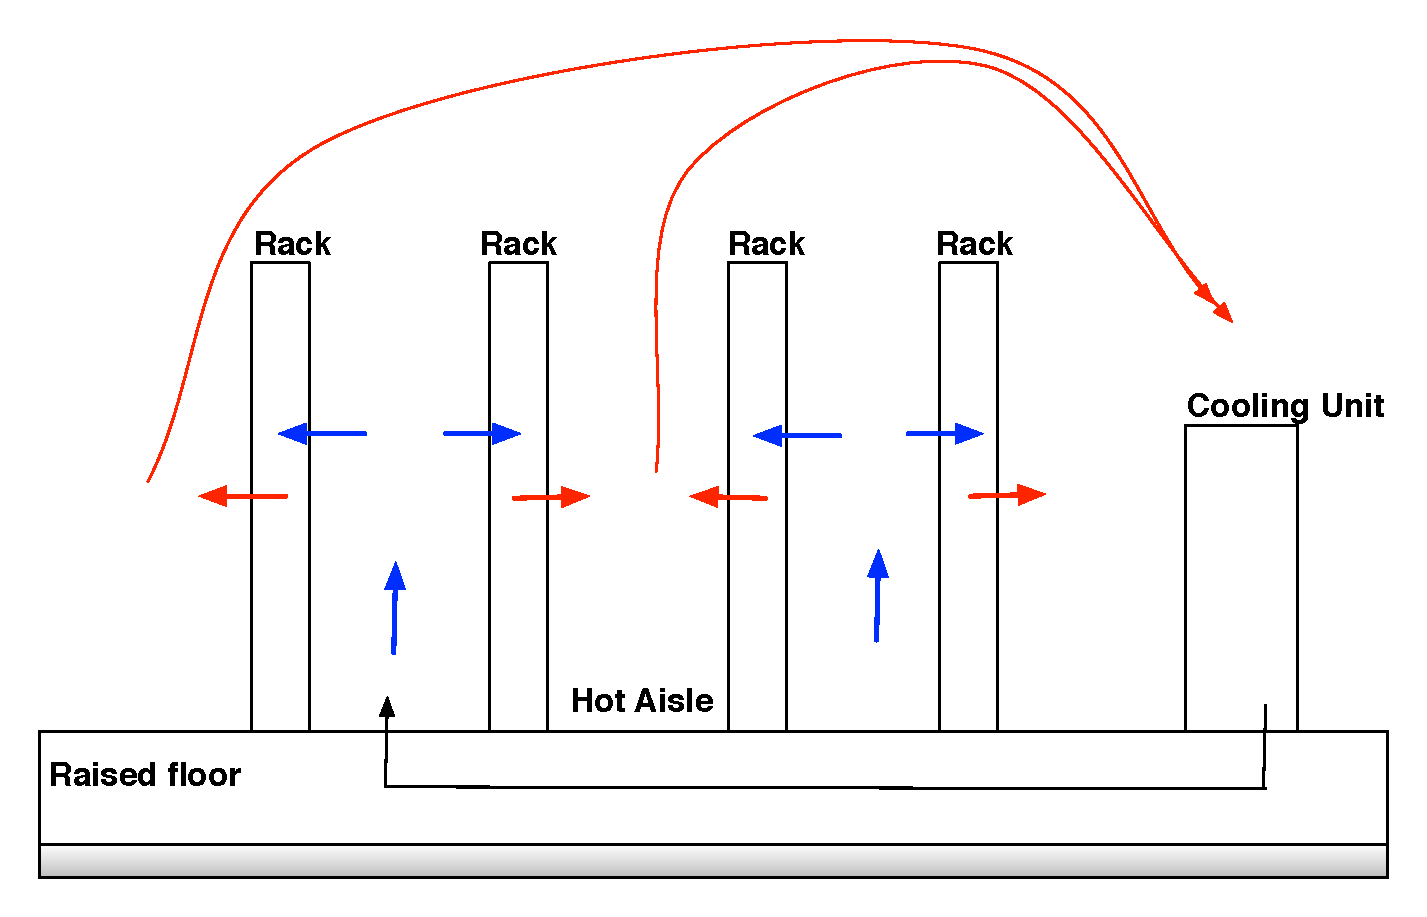
\includegraphics[scale=0.3]{graphs/datacenter.eps}
\end{center}
\caption{A typical data center schematic.
The cooling infrastructure comprises industry standard racks on a raised floor, through which multiple compressor-driven computer room air conditioning unit circulate cool air through a share plenum.}
\label{fig:twotier}
\vspace{-2mm}
\end{figure} 


\subsection{Thermodynamics of Data Center}\label{thermodynamics}
Data center seek to provision the cooling adequately to extract the heat produce by servers, switches, routers, and other devices.
Practically, cooling provisioning are done at facilities level.
Data center operator operate cooling facilities based on power ratings of servers, switches, routers, and other devices often with some additional headroom for risk tolerance. 
The compounded over provisioning of computing and cooling infrastructures can drive up initial and recurring costs. 
For every watt of power consumed by the computing infrastructure, a modern data center expends another one-half to one watt to power the cooling infrastructure \cite{}.

The cooling cycle of a typical data center operates in the following way:
Cooling units operate by extracting heat from the data center and pumping cold air into the room, usually through a pressurized floor plenum.
The pressure forces the cold air upward through vented tiles, entering the room in front the hardware
Fans draw the cold air inward and through the server; hot air exits through the rear of the server.
The hot air rises sometimes with the aid of fans and a ceiling plenum , and is sucked back to the cooling units.
The cooling units force the hot air past pipes containing cold air or water. 
The heat from the returning air transfer through the pipes to the cold substance. 
The heated substance leaves the room and goes to a chiller and cooling unit fans force the cold air back into the floor plenum. 

The efficiency of this cycle depends on several factors, including the conductive substance and the air flow velocity, but it is quantified by coefficient of performance (COP).
The COP is the ratio of heat removed ($Q$) to the amount of work necessary ($W$) to remove that heat:

\begin{eqnarray}\label{eqn:cop}
	COP=\frac{Q}{W}
\end{eqnarray}

Therefore, the work necessary to remove heat is inversely proportional to the COP.  
A higher COP indicates a more efficient process, requiring less work to remove a constant amount of heat.

However, the COP for a cooling cycling is not constant, increasing with the temperature of the air the cooling unit pushes into the plenum.  
COP value empirically can be computed using \cite{}:
\begin{eqnarray}\label{eqn:copt}
	COP(T) = 0.0068.T^2 + 0.0008.T + 0.458
\end{eqnarray}
where $T = T_{sup} + T_{adj}$ and $T_{adj} = T_{safe}^{in}-T_{max}^{in}$. \\
$T_{sup}$ is temperature supply by cooling unit and $T_{adj}$ is temperature difference between maximum safe server inlet temperature ($T_{safe}^{in}$) and the maximum observed server inlet temperature ($T_{max}^{in}$).
If $T_{adj}$ is negative, it indicates that a server inlet exceeds maximum safe temperature thus we need to lower $T_{sup}$ to bring the servers back below the system redline level.

\begin{figure}[thb]
\begin{center}
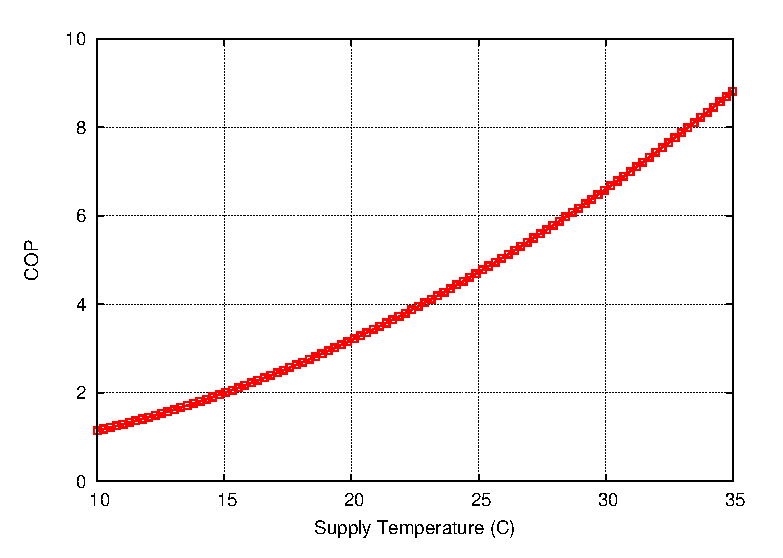
\includegraphics[scale=0.4]{graphs/cop.eps}
\end{center}
\caption{COP curve for the chilled water cooling units from HP Lab utility data center.
As the target temperature of the air the cooling unit pumps into the floor plenum increases, the COP increases.}
\label{fig:twotier}
\vspace{-2mm}
\end{figure} 


Cooling cost can be calculated as:
\begin{eqnarray}\label{eqn:cost}
C = \frac{Q}{COP(T)}
\end{eqnarray}
Where $Q$ is amount of power the servers and devices consume.
COP(T) is our COP at $T=T_{sup}+T_{adj}$.
Currently we assume a uniform $T_{sup}$ from each cooling units due to the complications introduced by non-uniform cold air supply.


\subsection{Energy Model}\label{energy model}
Power consumption model
\begin{equation}
	power(\lambda) = P_{idle} + (P_{peak}-P_{idle}). l 
\end{equation}
$0 \le l \le 1$ is the server load 

\section{Result and Analysis}\label{analysis}


\section{Related Work} 

Content Distribution Networks with peer assist have been successfully deployed on the Internet, such as Akamai \cite{Huang:2008:UHC:1496046.1496064} and LiveSky \cite{Yin:2010:LEC:1823746.1823750}.  
The authors of \cite{Huang:2008:UHC:1496046.1496064} conclude from two real world traces that hybrid CDN-P2P can significantly reduce the cost of content distribution and can scale to cope with the exponential growth of Internet video content.  
Yin et al. \cite{Yin:2010:LEC:1823746.1823750} described commercial operation of a peer-assisted CDN in China.  
LiveSky solved several challenges in the system design, such as dynamic resource scaling of P2P, low startup latency, ease of P2P integration with the existing CDN infrastructure, and network friendliness and upload fairness in the P2P operation.  
Xu et al.\cite{DBLP:journals/corr/abs-1212-4915} using game theory, showed that the right cooperative profit distribution of P2P can help the ISP to maximize the utility.  
Their model can easily be implemented in the context of current Internet economic settlements.  
Misra et al.\cite{Misra:2010:IPS:1811099.1811064} also mentioned the importance of P2P architecture to support content delivery networks.
The authors use cooperative game theory to formulate simple compensation rules for users who run P2P to support content delivery networks.

The idea of telco- or ISP-managed CDN has been proposed in recent years.  
The complexity of the CDN business encourage telcos and ISPs to manage their own CDN, rather than allow others to run CDNs on their networks.  
It has been shown that it is cost effective \cite{federation}\cite{norton2011internet}. 
Kamiyama et al. \cite{NoriakiKAMIYAMA2013} proposed optimally ISP operated CDN.
Kamiyama et al. mentioned that, in order to deliver large and rich Internet content to users, ISPs need to put their CDNs in data centers.  
The locations are limited while the storage is large, making this solution effective, using optimum placement algorithm based on real ISP network topologies.  
The authors found that inserting a CDN into an ISP's ladder-type network is effective in reducing the hop count, thus reduce total link cost.  
Cisco has initiated an effort to connect telco- or ISP-managed CDNs to each other, to form a CDN federation \cite{federation} using open standards \cite{cdni}.  
They argue that the current CDN architecture is not close enough to the users and ISPs can fill this position.

The idea of utilizing the user's computation power to support ISP operation is not new.  The Figaro project \cite{figaro} proposed residential gateway as an integrator of different networks and services, becoming an Internet-wide distributed content management for a proposed future Internet architecture \cite{figaro}.  
Cha e al.,\cite{Cha:2008:NTP:1855641.1855646} performed trace analysis and found that an IPTV architecture powered by P2P can handle a much larger number of channels, with limited demand for infrastructure compare to IP multicast.  
Jiang et al. \cite{Jiang:2012:OMD:2413176.2413193} proposed scalable and adaptive content replication and request routing for CDN servers located in users' home gateways.  
Maki et al.\cite{NaoyaMAKI2012} propose traffic engineering for peer-assisted CDN to control the behavior of clients, and present a solution for optimizing the selection of content files.
Mathieu et al., \cite{6249305} are using data gathered from France telecom network to calculate reduction of network load if customers are employed as peer-assisted content delivery.
Our work is same in system model architecture which uses different level of topologies  (Level-0 and Level-1), where in Mathieu et al., \cite{6249305} the authors use different names, which are regional and national. 
We emphasize that compare to  Mathieu et al., \cite{6249305} our work provides completely different approach.
Mathieu et al., \cite{6249305} work mostly based on empirical data from France telecom company thus the authors can directly calculate network load caused by video traffic and calculate network load reduction if peer-assisted is employed on customers side,  while our study focus on mathematical model of different admission policies for peers to join peer-assisted CDN and ISP payoff can get from employing peer-assisted CDN.


\section{Conclusion and Future Work}\label{conclusion}

This paper presents a scheme for a ISP managed peer-assisted CDN model that estimates lower bound of peers based on a stochastic fluid model and estimate the economic incentive for ISP based on game theory.
While a higher upload rate from the user nodes acting as seeders is desirable, it should be noted that an ISP should be aware of the implication that offering an economic incentive to too many users in order to get them acting as seeders in the P2P would have an undesirable effect on the ISP's revenue.
Some areas of improvement that we have identified for future are:
more work on the stochastic fluid model to include multiple video streaming bitrate and downtime effect of user home gateway and penalty to ISP payoff. 
We are also very interested to include energy trade off this peer-assisted CDN architecture in order to know how much energy saving by ISP and how much increase of energy at users home gateway side in this architecture.


\begin{acknowledgment}
We thank Rodney Van Meter for suggestions.
\end{acknowledgment}

\bibliographystyle{ipsjunsrt-e}% bib style
\bibliography{journal}% your bib database



\begin{biography}

\profile{Joho Taro}{was born in 1970. He received his M.S.\ degree from
 Johoshori University in 1994 and has been engaged in the Information
 Processing Society of Japan since 1994. His research interest is online
 publishing systems. He is a member of the IEEE and ACM\@.}
%
\profile{Shori Hanako}{was born in 1960. She received her M.E.\ and
 Ph.D.\ from Johoshori University in 1984 and 1987, respectively. She
 became an associate professor at Gakkai University in 1992 and a
 professor at Johoshori University in 1997. Her current research
 interest is online publishing systems. She received the Kiyasu Kinen
 award in 2010. She is a Board Member of the IPSJ and a member of the
 IEICE, IEEE-CS, and ACM\@.} 
%
\profile{Gakkai Jiro}{was born in 1970. He received his M.S.\ degree
 from Johoshori University in 1994 and has been engaged in the
 Information Processing Society of Japan since 1994. His research
 interest is online publishing systems. He is a member of the IEEE and
 ACM\@.}
%
\end{biography}
\end{document}
